\section{Study 1: How Does RePlay Support Activities in the Wild?}

A week-long field study with seven participants investigated whether and how people might use contextually-augmented video search in their own work. We focused on visual design, as videos are especially helpful for visual work \cite{Chi2012}.  Participants were recruited from the local design community and a prominent creative software company (\autoref{table:replay_study1_usage}). Participants had mixed amounts of experience with the main design software they used during the study (either Sketch or Adobe \textsc{xd}); all participants were proficient in at least one other creative application. Several had recently switched to Adobe \textsc{xd} or Sketch from other software, or had recently started their current job. After an initial interview, we installed RePlay on each participant's computer. Participants kept RePlay open throughout the next week while they worked (one used it for 10 days). Participants returned for a followup interview and received a \$45 gift card as compensation for their time. 

\begin{figure}[b!]
\centering
  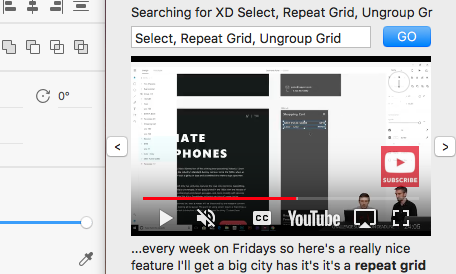
\includegraphics[width=.6\textwidth]{replay/figures/replay-old.png}
  \caption{Study 1 used this initial version of RePlay, shown here next to Adobe \textsc{xd}. It did not show video titles or timeline markers; instead it had arrow buttons next to each video to skip between that video's ranked clips. It also added the 3 most recent tools to the search field instead of one. }~\label{fig:replay-old}
%   \Description[A screenshot of an older version of RePlay.]{A screenshot of an older version of RePlay. Above the search field, the status area reads ``Searching for XD Select, Repeat Grid, Ungroup Grid''. Inside the search field it reads ``Select, Repeat Grid, Ungroup Grid''. It displays a video result with no title and a short caption excerpt underneath that includes the words ``repeat grid'' bolded.}
\end{figure}

Participants used an initial version of RePlay (\autoref{fig:replay-old}); based on their feedback, we revised it to the version presented in the previous section. Study 1's RePlay did not consider cross-application context; it only used context from the current application. This RePlay only monitored Adobe \textsc{xd} and Sketch to avoid capturing unrelated or private data from other applications. RePlay logged the following events to the custom server when it was open: all clicks on interface elements in Adobe \textsc{xd} and Sketch, all interactions with RePlay, and all switches to and between other applications.

We took notes on all interviews, noting similar answers to questions and identifying common themes. This data and feedback helped motivate the final version's focus on cross-application support, helped us understand what kinds of tasks RePlay may be most useful for, and highlighted some advantages and challenges of contextual support.

\subsection{Results}
Over the week, participants reported spending between 1.5 and 30 hours on their design work (\autoref{table:replay_study1_usage}). Some said they kept RePlay open the entire time; others closed it at times to focus on their work. 

Generally, participants appreciated having help readily available. As \textit{P2} explained, \textit{``this gives me an interface where I can search and do everything and it's automatically there right next to the design. There are no extra steps.''} \textit{P4} enjoyed seeing RePlay react to her actions: \textit{``it felt like I had a buddy.''} Only one (\textit{P6}, the expert) did not use it at all: he was fluent in the software and did not seek assistance.

\subsubsection{Contextual clip search was most useful for specific tasks}
Four participants said they tended to use RePlay when stuck trying to figure out how to do something specific. Three also said they used it to find out what a particular tool could do or how to use it. All but one participant worked on targeted tasks (see \autoref{table:replay_study1_usage}). \textit{P3} wanted general resources for getting started with Sketch, and did not find RePlay helpful.

\begin{table*}[t]
\centering
\caption{Study 1 participant background and usage. Participants self-reported their experience, design work done, hours spent designing, and \% of that time with RePlay open. \# queries and \# videos watched were calculated from RePlay's usage data. }~\label{table:replay_study1_usage}
\resizebox{1\textwidth}{!}{
\begin{tabular}{lllllcccc}
\multicolumn{1}{l}{} & \textbf{Job title} & \textbf{Main app} & \textbf{\begin{tabular}[c]{@{}l@{}}Experience\\ w/ app\end{tabular}} & \textbf{Design work done} & \textbf{\begin{tabular}[c]{@{}l@{}}Hours\\ designing\end{tabular}} & \multicolumn{1}{l}{\textbf{\begin{tabular}[c]{@{}l@{}}Time w/\\ RePlay open\end{tabular}}} & \multicolumn{1}{l}{\textbf{\begin{tabular}[c]{@{}l@{}}\# queries\end{tabular}}} & \multicolumn{1}{l}{\textbf{\begin{tabular}[c]{@{}l@{}}\# videos \\ watched\end{tabular}}} \\
\textit{P1}          & Sr. Product Manager   & Adobe \textsc{xd}     & Beginner      & Style guide and wireframing                                                  & 20                                                                            & 100\%                                                                                          & \phantom{0}3                    & 4                                                                                         \\
\textit{P2}          & Freelance Designer       & Adobe \textsc{xd}     & Beginner      & Wireframing / prototype design                                               & 4.5                                                                           & 100\%                                                                                         & 10                   & 5                                                                                         \\
\textit{P3}          & Freelance Designer       & Sketch                & Beginner      & Trying to learn Sketch                                                       & 1.5                                                                           & 100\%                                                                                         & \phantom{0}4                    & 2                                                                                         \\
\textit{P4}          & PhD Student              & Sketch                & Intermediate  & Screen design and grid customizing                                           & 5                                                                             & 40\%                                                                                            & 10                   & 0                                                                                         \\
\textit{P5}          & UX Designer              & Sketch                & Beginner      & Creating templates and logos                                                 & 30                                                                            & 70\%                                                                                           & 24                   & 8                                                                                         \\
\textit{P6}          & Sr. UX Designer       & Adobe \textsc{xd}     & Expert        & UX workflows                                                                 & 20                                                                            & 25\%                                                                                            & \phantom{0}0                    & 0                                                                                         \\
\textit{P7}          & Sr. UX Designer       & Adobe \textsc{xd}     & Intermediate  & Wireframing an app UI                                                        & 12                                                                            & 33\%                                                                                            & 19                   & 13\phantom{0}                                                                                       
\end{tabular}
}
\end{table*}

Three users recounted similar stories of searching for a particular question and quickly finding a clip within a video that answered it. \textit{P1} described searching for ``Make Symbol'' after clicking on the ``Make Symbol'' tool in Adobe \textsc{xd}. The answer he needed came from an auto-selected moment near the end of a 3-hour video. \textit{P1} added, \textit{``if I had searched for that myself I would've given up.''} Similarly, \textit{P5} found what he needed in a 1.5-hour video that was cued to a moment 20 minutes in. He was trying to create margins, searched for ``layout grid'', and \textit{``the first video in the list showed me exactly what I needed to do''}, which was to check a box he hadn't noticed. \textit{P4} found RePlay useful for indicating that her specific goal was \textit{not} possible: she wanted to customize a grid system in Sketch and searched for ``grid settings'', but the caption excerpts indicated that none of the results mentioned customizing grids.

Contextual video clips sometimes invited opportunistic learning: \textit{P1} and \textit{P7} recounted instances where a video they were watching taught them something they didn't know and hadn't thought to look for. \textit{P1} continued watching the ``make symbols'' video as it described grouping and layering symbols. This part \textit{``wasn't originally what I was searching for but it was exactly what I needed ... [I] gained a lot more knowledge.''} \textit{P7} described how he \textit{``searched for `character styles' and actually found new information that I've never seen before''} about the Libraries panel.

%\vspace{0.1in}
\subsubsection{Tool context helps, but not in the search query}
All participants who searched with RePlay preferred deleting tool names from the search field and instead typing their own. Five participants mentioned that including three tools in the query was too many, as it made the query too general. \textit{P3} said the automatic query seemed \textit{``stuck on the last thing I did, which might not be relevant to what I'm thinking now.''} Both \textit{P4} and \textit{P5} said tool \textit{names} were not as useful because they wanted to search for an \textit{action}, not its constituent tools (\textit{e.g.,} ``rotate object'' or ``export nested artboard''). Higher-level activity inference may provide more useful assistance.

Two participants said they liked that RePlay populated the query with tool names because \textit{``coming up with the right search terms is really hard and I don't know the names of the tools [...] so it's nice not to have to think of them''} (\textit{P4}). Even \textit{P6}, the expert, said \textit{``I know how to use everything but if you asked me the names of the tools, I have no idea}.'' Participants appreciated that RePlay added the application name to the query, as it allowed them to \textit{``spend more brain power on the details of [the query]'' (P2)}. 

\subsubsection{Participants frequently switched between applications}
RePlay logged every time users switched between \textit{any} applications when it was running. Excluding system applications (such as Dock, Finder, and System Preferences), participants used an average of 17 different applications while RePlay was running ($SD\!=\!8$), and switched between applications a mean of every 6.6 minutes ($SD\!=\!8.5$min). If we exclude all continuous periods of over 3 hours (assuming that these sessions were breaks of some sort), this average lowers to every 2.5 minutes ($SD\!=\!1.8$min). This diverse application usage supports our motivation for improving cross-application workflows.

\subsubsection{Improvements to RePlay}
Because participants thought that automatically including three tools was too many, Replay now includes only the most recent one. Four participants also mentioned that more general information like video titles would be helpful, as caption excerpts often seemed \textit{``out of context''} or \textit{``snatched out of middle of a sentence''} (\textit{P2}). Consequently, RePlay now includes video titles. Four participants wished they could watch videos at a larger size; RePlay now includes a resizable video player window. Two participants also mentioned that some video results did not pertain to the current application; RePlay now excludes results that do not mention the current application in the metadata or captions.
